\chapter{Implementation}

\section{Repository}

\subsection{Repository and Contribution}

\begin{itemize}
    \item \mintinline{bash}{src/}
    \begin{itemize}
        \item \mintinline{bash}{compiler/qccd_color_qubits_to_ions.py}: code for topology aware color code qubit mapping.
        \item \mintinline{bash}{simulator/}
        \begin{itemize}
            \item \mintinline{bash}{qccd_circuit.py}: code contributions to adapt framework for color code generation and decoding compatibility for the simulation
            \item \mintinline{bash}{color_code_processor.py}: code used to process and compile color codes
        \end{itemize}
    \end{itemize}

    \item \mintinline{bash}{color_code_utils/}
    \begin{itemize}
        \item \mintinline{bash}{color_code_circuits/} folder containing implementations of various experimental color codes, including the main (6.6.6) implementation in \mintinline{bash}{color_code_circuit_666.py}

        \item \mintinline{bash}{abstract_color_code_circuit.py}, \mintinline{bash}{color_code_tile.py} helper classes and templates for color code circuit implementations
    \end{itemize}

    \item \mintinline{bash}{color_code_experiments/} Jupyter notebooks for testing, plot generation, research and experimentation based tasks

    \item \mintinline{bash}{data/cc_data/} folder containing results and outputs from color code compilation simulations
    
    \item \mintinline{bash}{tests/}

    \item \textit{config\_model.yml}, \textit{config\_color.yml}: configuration files to specify parameters for compiler runs
    
\end{itemize}
Give the clearest respository overview the world has ever seen, including a clear diagram and indication of where the relevant implementation sections are and why.

\section{Implementing Color Code Circuits}
\label{sec:impl_color_code}

The first milestone of this project was to produce a set of color code circuits that could be used to compile onto QCCD architecture. This was motivated by the lack of native color code circuit support in stim, meaning the project required developing alternative, new chromobius compatible color code circuits in stim for the compilation pipeline.

\subsection{(6.6.6) Color Code Topology}

As mentioned in the preparation chapter, color codes require a three-colourable tiling that can manifest as 3 possible tessellations. The (4.8.8), the (6.6.6) and the (4.6.12), each defining a distinct triangular color code topology \cite{landahl2011faulttolerantquantumcomputingcolor}. 

\begin{figure}[!h]
    \centering
    \includegraphics[width=0.75\linewidth]{assets/colorcodetessellations.png}
    \caption{The three possible tilings of a triangular color code, each of distance 11 from \cite{landahl2011faulttolerantquantumcomputingcolor}}
    \label{fig:colorcodetessellations}
\end{figure}
Of these, the (6.6.6) was an ideal candidate for implementation due to its relatively simpler topology and richer source of documentation and literature, enabling faster development towards a working prototype. 

The (6.6.6) triangular color code produces a uniform tiling made of hexagons and half-hexagons in an equilateral triangle. For this, a \mintinline{python}{ColorCodeCircuit666} class was developed, alongside a function \mintinline{python}{_generate_layout()} constructing the required hexagonal lattice for a given distance, defining data qubits at each vertex and a central ancilla qubit for each plaquette.

A specific design decision in this implementation was the use of a single ancillary qubit per face for stabilizer measurement (demonstrated in Fig. \ref{fig:circuitschedule}). Although this approach increased the total number of circuit operations due to reduced parallelism in the extraction of stabilizer syndromes, it was chosen to provide ease of debugging during development. Prioritizing a much simpler measurement schedule enabled incremental validation of the circuit and its schedule, which was particularly valuable at this early stage of the project.

There exist more sophisticated and complex scheduling strategies and architectural implementations, which have been shown to achieve improved fault-tolerance thresholds \cite{chromobius, flaggedweightcolorcode}, but the main objective of this section was rapid prototyping to be able to devote more attention to the compilation stages.
-> could talk abt research finding more optimal schedules
\begin{figure}[!h]
    \centering
    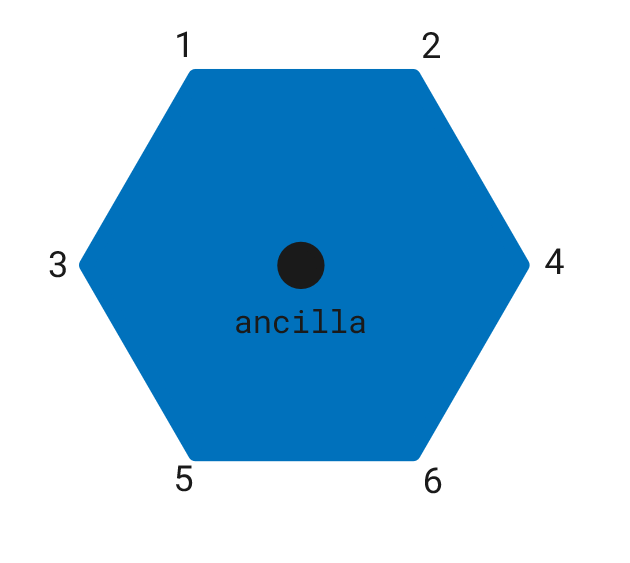
\includegraphics[width=0.325\linewidth]{assets/hexagon.png}
    \caption{Example plaquette and numbering corresponding to circuit schedule in Fig \ref{fig:circuitschedule}}
    \label{fig:hexagon}
\end{figure}

\begin{figure}
    \centering
    \begin{quantikz}
        \lstick{1} &&\targ{}&&&&&& &&\ctrl{3}&&&&&& &\\
        \lstick{2} &&&\targ{}&&&&& &&&\ctrl{2}&&&&& &\\
        \lstick{3} &&&&\targ{}&&&& &&&&\ctrl{1}&&&& &\\
        \lstick{a} & \gate{RX} &\ctrl{-3} &\ctrl{-2} &\ctrl{-1} &\ctrl{1}&\ctrl{2}&\ctrl{3} & \gate{MX} & \gate{RZ} &\targ{} &\targ{} &\targ{} &\targ{}&\targ{}&\targ{} & \gate{MZ} & \\
        \lstick{4} &&&&&\targ{}&&& &&&&&\ctrl{-1}&&& &\\
        \lstick{5} &&&&&&\targ{}&& &&&&&&\ctrl{-2}&& & \\
        \lstick{6} &&&&&&&\targ{}& &&&&&&&\ctrl{-3}& & \\
    \end{quantikz}
    \caption{Measurement schedule for a color code circuit with a single ancilla qubit}
    \label{fig:circuitschedule}
\end{figure}


\subsection{Generating the Circuit}

Typically, a stabilizer code circuit involves iterations of stabilizer measurement and defining detectors between cycles (demonstrated in Fig \ref{fig:stabilizerscircuit}). Detectors in stim are used to provide explicit annotations that define which combination of measurement results should be parity checked to find the presence of an error. This enables measurement outcomes to be compared between consecutive rounds in the circuit such that detection events (changes in the stabilizer values) can be identified, suggesting the occurrence of errors. 

\begin{figure}[!h]
    \centering
    \begin{quantikz}
        & \gate[4]{\text{X stabilizers}} & \gate[4]{\text{Z stabilizers}} & \gate[4]{\text{Detectors}} & \gate[4]{\text{X stabilizers}} & \gate[4]{\text{Z stabilizers}} & \gate[4]{\text{Detectors}} &\\
        & & & & & & &\\
        {\vdots}  \\
        & & & & & & &\\
    \end{quantikz}
    \caption{Example timeline of measuring the X and Z stabilizers in a color code}
    \label{fig:stabilizerscircuit}
\end{figure}

Taking the tiles generated from the \mintinline{python}{_generate_layout()}, \mintinline{python}{_build_circuit()} was written to construct the stim circuit, using helper functions \mintinline{python}{_measure_rounds()} and \mintinline{python}{_measure_stabilizers()} to model the qubit-level operations per stabilizer measurement and include the detector annotations required by chromobius into the stim circuit. To guide my construction process, Refs. \cite{flaggedweightcolorcode, landahl2011faulttolerantquantumcomputingcolor} were examined for the default single-qubit syndrome extraction models that detailed operation schedules for a single ancilla color code.

\subsection{Noise Model}

The noise model for a quantum circuit is used to characterise the types and distribution of errors that may occur during the operation of the circuit, mapping ideal unitary operations to noisy channels. 

Several noise models exist in literature which vary in levels of abstraction, starting with the code-capacity noise model assuming independent errors on only data qubits between perfect syndrome measurements. The phenomenological noise model introduces additional complexity of faulty syndrome extraction where measurement outcomes are also subject to error. Finally, the circuit-level noise model assigns individual error probabilities to each physical operation.

With a focus on realistic modelling and compilation of color codes onto QCCD architecture, the noise model chosen for this implementation was the circuit-level noise model, selected to capture the detailed error mechanisms that may occur during the execution of a circuit.

The circuit-level noise model of strength $p$ involve the following operations, alongside their respective stim interfaces that are used to model them:
\begin{itemize}
    \item Idle qubits (identity gate) or single qubit gates act ideally, followed by a single-qubit depolarizing noise channel: \newline(\mintinline{python}{DEPOLARIZE_1(p) q})
    \item Two qubit gates act ideally, followed by a two-qubit depolarizing noise channel: \newline(\mintinline{python}{DEPOLARIZE_2(p) q1 q2})
    \item On measurement, the result may be flipped with probability $p$: \newline(\mintinline{python}{M(p) q/MX(p) q})
    \item State preparation/resets may produce an orthogonal state with probability $p$: \newline(\mintinline{python}{X_ERROR(p)/Z_ERROR(p) q})
\end{itemize}

The single qubit depolarizing channel is defined as:
\begin{align}
    \varepsilon^1(p): (1-p) &\mapsto I\\
    p/3 &\mapsto X\\
    p/3 &\mapsto Y\\
    p/3 &\mapsto Z\\
\end{align}

The two-qubit depolarizing channel is defined as:
\begin{align}
    \varepsilon^1(p): (1-p) &\mapsto I\otimes I\\
    p/15 &\mapsto P_1\otimes P_2  & (\forall P_1,P_2 \in \{I,X,Y,Z\}\text{ where } (P_1,P_2) \neq (I,I))
\end{align}

\section{Qubit Mapping}
\label{sec:impl_qubit_mapping}

Once the color code circuit is generated, the compiler must map the qubits to physical ions within traps in the QCCD architecture. This process makes use of a two-step pipeline: qubit clustering followed by cluster to trap mapping. 
The primary architectural challenge of compiling color codes lies in their high weight stabilizer generators and triangular lattice that differs from surface codes. Therefore, this project will focus exclusively on developing and evaluating novel clustering methodologies for color codes. The subsequent mapping of these clusters to physical traps is handled by the base framework \cite{scottPaper}, a deliberate choice to isolate the topology-aware mapping challenge from the hardware-specific trap assignment.

Abstractly, qubit clustering can be modelled as a balanced graph partitioning problem, where given a graph $G = (V,E)$ with $V$ as qubits and edges in $E$ representing the two-qubit interactions in the circuit, $V$ should be divided into roughly $k$ equal-sized clusters whilst minimising the number of cut edges.
However, balanced graph partitioning is considered NP-complete, where no poly-time approximation algorithm can guarantee a finite approximation ratio unless $P=NP$ \cite{balancedGraphPartitioning}. Instead, a heuristic based methodology must be employed, exploiting topology to preserve qubit neighbourhoods during clustering and minimising ancilla movements between ion traps.

Choosing an appropriate cluster capacity is important at this stage, as this can influence the ion routing schedule between traps. Having the cluster size equal to the trap capacity can overly restrict movement and parallelism of operations as an ion must first be displaced from a trap for another ion to enter it. However, a sparse trap can unnecessarily increase the number of ion routing operations. For this reason, this project utilises a clustering capacity equal to $\textbf{trap capacity} - 1$.

\subsection{Triangular Mapping Strategy}

To map the triangular color code onto the physical hardware, one viable heuristic is to take advantage of its natural geometric topology. The core idea behind this mapping strategy being to group the physical qubits (ions) into distinct clusters by recursively subdividing the spatial area they occupy.

Inspired by the Sierpinski triangle, the algorithm first bounds the entire array of ions within a single large outer triangle. The space is then subdivided into four sub-triangles (visualised in Fig. \ref{fig:triclustering}). The division process is repeated on the sub-triangles until the number of ions within a given triangle falls below a given clustering threshold.

\begin{figure}[!h]
    \centering
    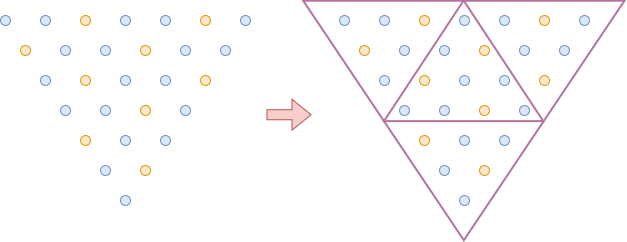
\includegraphics[width=0.75\linewidth]{assets/triclustering.png}
    \caption{Clustering mechanic for a triangular topology using an example distance 5 (6.6.6) color code with data qubits (blue) and ancilla qubits (yellow)}
    \label{fig:triclustering}
\end{figure}

The subdivision of points occupying a triangular area can be done by converting the position of each point into barycentric coordinates and classifying the point into a sector of the triangle. For a point in the triangle defined by vertices $A$, $B$ and $C$, the barycentric coordinates can be given as a linear combination of these vectors

\begin{equation} 
    p = uA + vB + wC,
\end{equation}
with the constraint that 
\begin{equation}
    u + v + w = 1, \;\; u\geq 0, v\geq 0, w\geq 0
\end{equation}

\begin{figure}[!h]
    \centering
    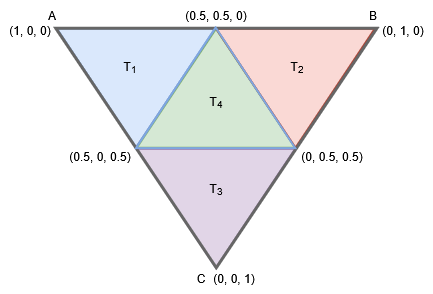
\includegraphics[width=0.75\linewidth]{assets/barycentricTriangle.png}
    \caption{Sub-triangles defined within the barycentric coordinate space of the outer triangle with points and their respective coordinates defined in terms of $\triangle ABC$}
    \label{fig:barycentric}
\end{figure}

The core logic for this spatial clustering approach, outlined in Alg. \ref{alg:tri_clustering}, uses an iterative, queue-based breadth-first search to perform partitioning steps. At each iteration, the algorithm calculates the edge midpoints of the current triangle's edges to define the four nested sub-triangles. Qubits within the parent region are then mapped to sub-regions using their barycentric coordinates. This subdivision process continues until the number of unassigned qubits within a sub-triangle falls below the maximum trap capacity constraint.

\begin{algorithm}
\caption{Triangular Clustering Algorithm}
\label{alg:tri_clustering}
\begin{algorithmic}[1]
    \REQUIRE Point set $X$, max capacity of $k$
    \ENSURE Set of final merged clusters $\mathcal{C}_{final}$ such that $\forall C \in \mathcal{C}_{final}.\; |C|\le k$
    
    \STATE $T_{root} \leftarrow \text{Bounding triangle enclosing } X$
    \STATE $Q \leftarrow \text{Queue initialized with } (T_{root}, X)$
    \STATE $\mathcal{C} \leftarrow \emptyset$ \COMMENT{Set of initial clusters}
    
    \WHILE{$Q$ is not empty}
        \STATE Dequeue $(T, P)$ from $Q$
        
        \IF{$|P| \le k$}
            \STATE $\mathcal{C} \leftarrow \mathcal{C} \cup \{P\}$
            \STATE \textbf{continue}
        \ENDIF
        
        \STATE Partition $T$ into four congruent subtriangles $\{T_1, T_2, T_3, T_4\}$ via edge midpoints
        \STATE Partition $P$ into subsets $\{P_1, P_2, P_3, P_4\}$ such that $p \in P_i$ if $p$ lies within $T_i$
        
        \FOR{$i \in \{1, 2, 3, 4\}$}
            \IF{$|P_i| > 0$}
                \STATE Enqueue $(T_i, P_i)$ onto $Q$
            \ENDIF
        \ENDFOR
    \ENDWHILE
    
    \STATE $\mathcal{C}_{final} \leftarrow \text{MergeUnderfilledClusters}(\mathcal{C}, k)$
    \RETURN $\mathcal{C}_{final}$
\end{algorithmic}
\end{algorithm}


Given that the exact triangular shape of the color code may change depending on the specific tessellation being used, a necessary design objective was to ensure the algorithm remained flexible for different bounding triangles.
By defining partition boundaries strictly through edge midpoints rather than rigid geometric properties (e.g. fixed angles or side lengths), the clustering methodology maintains compatibility across arbitrary triangular lattice layouts. 

Assuming a relatively uniform distribution of $N$  input qubits, each subdivision partition the points into four subsets, resulting in a partitioning tree depth of $\log_4 (N)$. The implementation uses vectorised NumPy operations to evaluate barycentric coordinates. The algorithm therefore performs the processing of all points at any given depth in $O(N)$ time. As a result, the average-case time complexity is bounded at $O(N\log N)$. Since the initial bounding triangle is defined using the input set of points, our assumption should usually hold.
Additionally, worst-case space complexity is $O(N)$, since the BFS queue will at most store references to all $N$ coordinates during a partitioning cycle.

\subsubsection{Preventing Overclustering}

While the triangular partitioning effectively groups ions based on the color code's natural topology, its strict geometric clustering has a critical flaw, where it can produce sparse or ``underfilled'' clusters due to the four-way splitting mechanism, often near the edges of the lattice, leaving these ions isolated in their own traps. This can have a significant effect on ion routing, resulting in inefficient schedules and therefore, longer end-to-end runtimes and higher error rates during compilation.

To resolve this, a merging phase is applied to the clusters. The core idea is to prioritize the smallest clusters and combine them with their neighbors. To do this, the algorithm sorts the clusters by size and searches the vicinity of each underfilled cluster. If combining a small cluster with a nearby neighbor keeps the total number of ions below the trap's maximum capacity, the two clusters are merged into one.

Several merging methods (which influence the neighbours that are considered) were explored, including:
\begin{itemize}
    \item Bounded distance merging
    \item Unbounded cluster merging
    \item $k$-nearest-neighbour merging
\end{itemize}

For bounded distance merging, experimental thresholds around the maximum distance between neighbouring ancilla qubits, 

\begin{equation}
    \text{thresh} = \max_{i,j}\; \text{distance}(a_i, a_j),  
\end{equation}
were explored to preserve high locality in the clustering. As $\text{thresh} \rightarrow \infty$, this method degrades to an unbounded distance search strategy. 

The generalized logic for this bottom-up approach is outlined in Alg. \ref{alg:merge_clusters}. The procedure iteratively searches for the closest valid partner for the smallest active clusters. Once a successful merge occurs, the cluster lists are updated, and the process repeats until no further merges can be made.
 
\begin{algorithm}
\caption{Greedy Merging of Underfilled Clusters}
\label{alg:merge_clusters}
\begin{algorithmic}[1]
    \REQUIRE Initial set of clusters $\mathcal{C}$, max cluster capacity $k_{max}$
    \ENSURE Final set of merged clusters $\mathcal{C}_{final}$
    
    \STATE $merged \leftarrow \text{True}$
    
    \WHILE{$merged$ is True and $|\mathcal{C}| \ge 2$}
        \STATE $merged \leftarrow \text{False}$
        \STATE Sort $\mathcal{C}$ in ascending order based on cluster size $|c|$
        
        \FOR{\textbf{each} cluster $c_i \in \mathcal{C}$}
            \STATE Find candidate neighbours $\mathcal{N}(c_i)$ \COMMENT{e.g., via $k$-NN or radius threshold value}
            \STATE Initialize $c_{best} \leftarrow \text{null}$, $d_{min} \leftarrow \infty$
            
            \FOR{\textbf{each} candidate $c_j \in \mathcal{N}(c_i)$}
                \IF{$|c_i| + |c_j| \le k_{max}$}
                    \STATE $d \leftarrow ||\mu_{c_i} - \mu_{c_j}||$
                    \IF{$d < d_{min}$}
                        \STATE $d_{min} \leftarrow d$
                        \STATE $c_{best} \leftarrow c_j$
                    \ENDIF
                \ENDIF
            \ENDFOR
            
            \IF{$c_{best} \neq \text{null}$}
                \STATE $c_{new} \leftarrow c_i \cup c_{best}$ \COMMENT{Combine ion coordinate sets}
                \STATE $\mu_{new} \leftarrow \frac{|c_i|\mu_{c_i} + |c_{best}|\mu_{c_{best}}}{|c_i| + |c_{best}|}$ \COMMENT{Size-weighted center of mass}
                
                \STATE $\mathcal{C} \leftarrow (\mathcal{C} \setminus \{c_i, c_{best}\}) \cup \{c_{new}\}$
                \STATE $merged \leftarrow \text{True}$
                \STATE \textbf{break}
            \ENDIF
        \ENDFOR
    \ENDWHILE
    
    \RETURN $\mathcal{C}$
\end{algorithmic}
\end{algorithm}

The algorithm was modified to implement the different merging strategies mentioned above, yielding different final clusters and overall compilation results (discussed in Section \ref{sec:qubit_mapping_eval}).

A particularly useful data structure in this implementation was the use of a KD-tree, a binary search tree in $k$-dimensional space with $N$ items, enabling fast $O(\log N)$ lookups of cluster centers for operations relating to line 6 in Alg. \ref{alg:merge_clusters}. 

Suppose the input to the merging algorithm are $K$ clusters. Analysing a single iteration of the while loop, initialisation of a KD-tree takes $O(K \log K)$. The sorting of the active clusters by size also takes $O(K \log K)$. The KD-tree is then queried for the nearest neighbour(s) (depending on the strategy), resulting in a query time of at most $O(K \log K)$.
In the worst case scenario, the algorithm finds one valid merge per while-loop iteration requiring a rebuild of the KD-tree each iteration, causing the loop to run $O(K)$ times and producing a total time complexity of $O(K^2\log K)$. Considering that $K$ is often significantly smaller than $N$, where $N$ is the number of qubits, the effect of the merging process on the execution time of the overall clustering mechanism is almost negligible.


\subsection{Clustering Comparisons}

Clustering results were frequently tested and compared between the framework implementation and the project's triangular clustering with different merging strategies. 

A visualisation of each clustering mechanism is given on the (6.6.6) color code of distance 5 at trap capacities 5 and 10, grouping clusters by colour alongside their centroids indicated in the plot by $\times$.

\subsubsection{Trap capacity 5:} 

\begin{figure}[H]
    \centering
     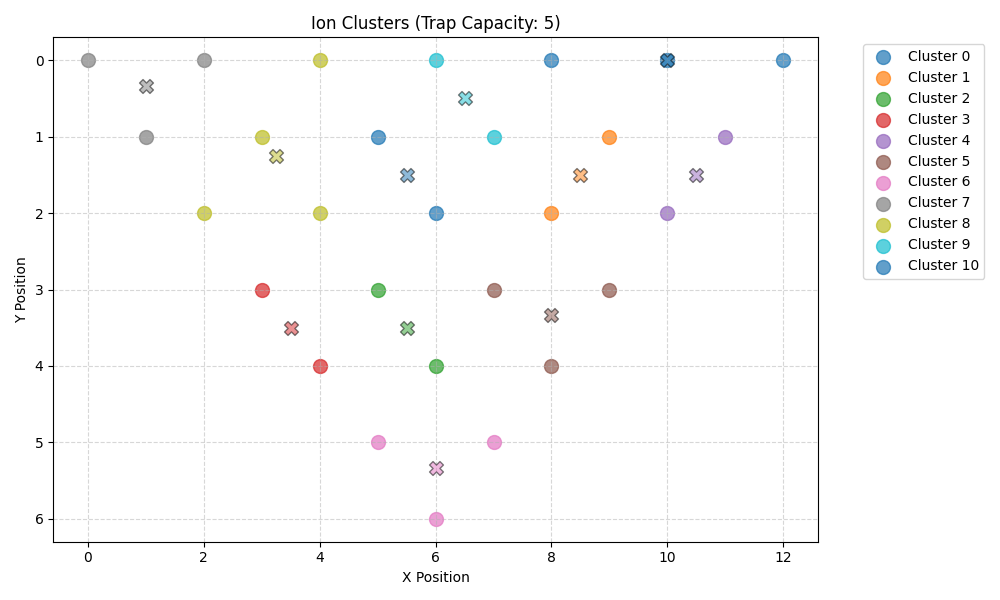
\includegraphics[width=\textwidth]{assets/clusters/halving_clusters_tc=5_d=5.png}
     \caption{Framework clustering mechanism}
     \label{fig:plot1}
\end{figure}

\begin{figure}[H]
    \centering
     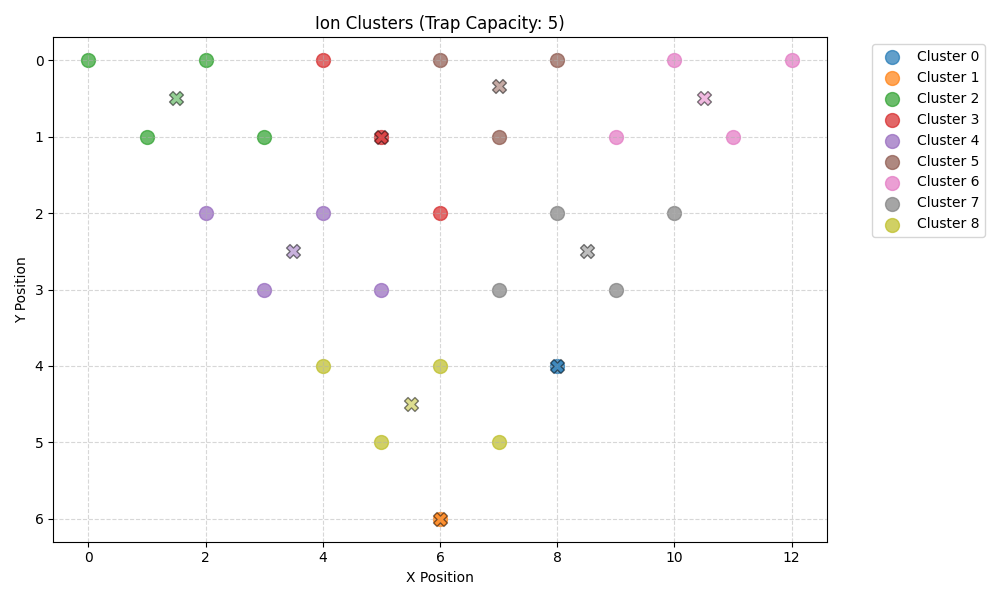
\includegraphics[width=\textwidth]{assets/clusters/tri_dist_bounded_nn_clusters_tc=5_d=5.png}
     \caption{Bounded nearest-neighbour clustering, $\text{thresh} = 2.5$}
     \label{fig:plot2}
\end{figure}

\begin{figure}[H]
    \centering
     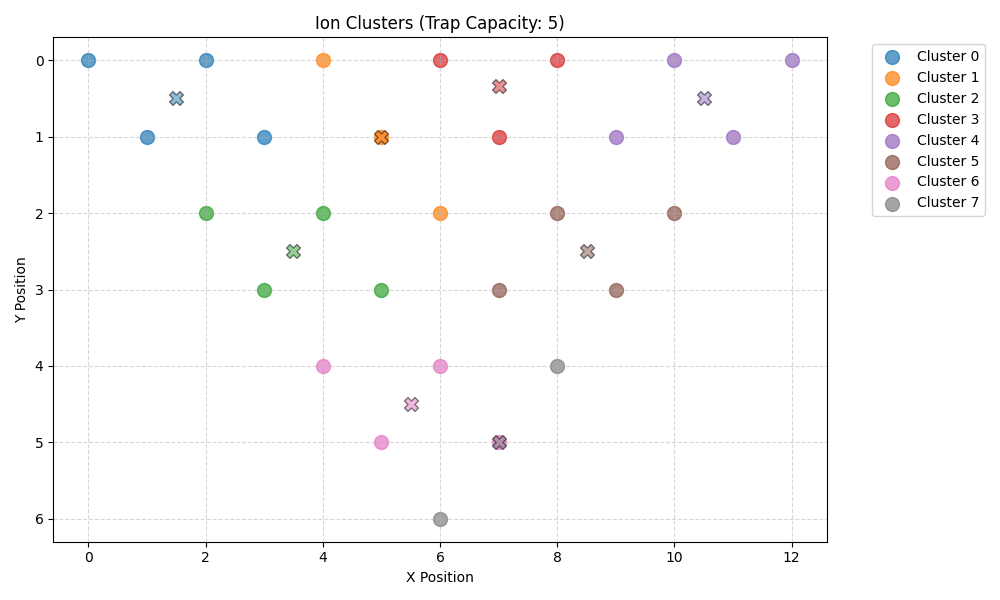
\includegraphics[width=\textwidth]{assets/clusters/tri_knn_clusters_tc=5_d=5.png}
     \caption{$k$-nearest-neighbour clustering, $k=3$}
     \label{fig:plot3}
\end{figure}

\begin{figure}[H]
    \centering
     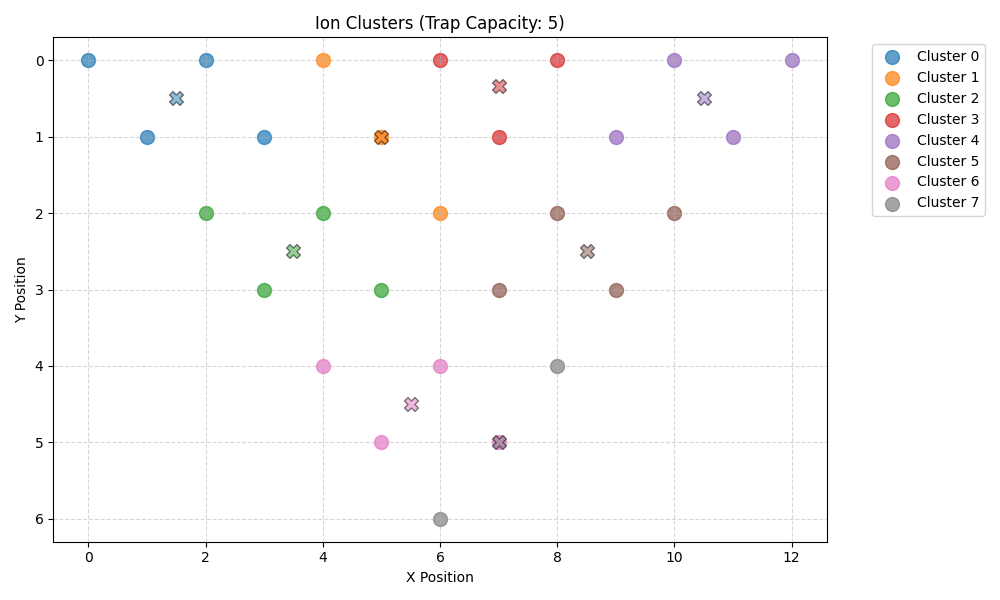
\includegraphics[width=\textwidth]{assets/clusters/tri_unbounded_nn_clusters_tc=5_d=5.png}
     \caption{Unbounded nearest-neighbour clustering}
     \label{fig:plot4}
\end{figure}

\subsubsection{Trap capacity 10:}

\begin{figure}[H]
    \centering
     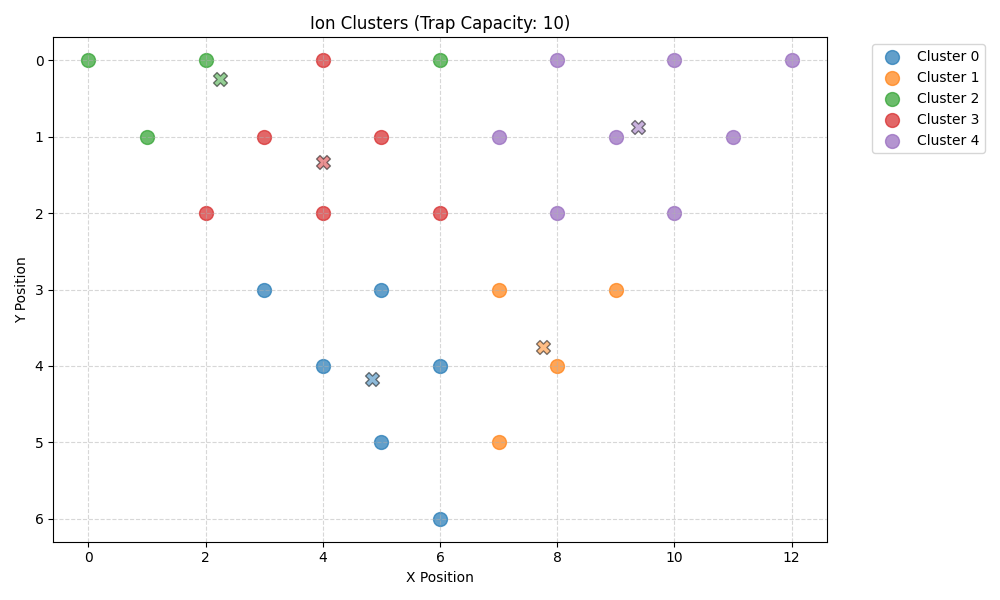
\includegraphics[width=\textwidth]{assets/clusters/halving_clusters_tc=10_d=5.png}
     \caption{Framework clustering mechanism}
     \label{fig:framework10}
\end{figure}

\begin{figure}[H]
    \centering
     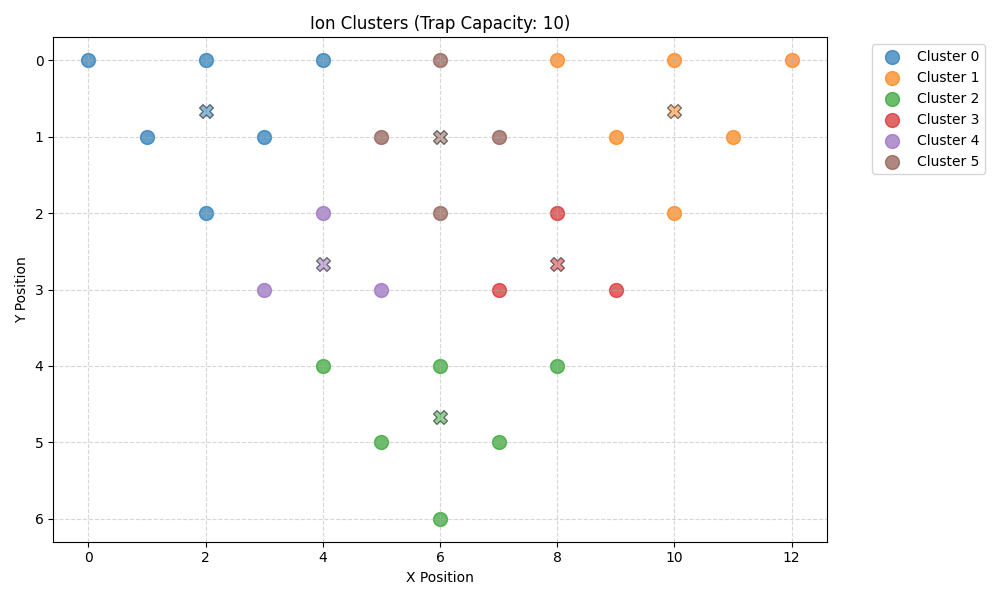
\includegraphics[width=\textwidth]{assets/clusters/tri_dist_bounded_nn_clusters_tc=10_d=5.png}
     \caption{Bounded nearest-neighbour clustering, $\text{thresh} = 2.5$}
     \label{fig:plot2}
\end{figure}

\begin{figure}[H]
    \centering
     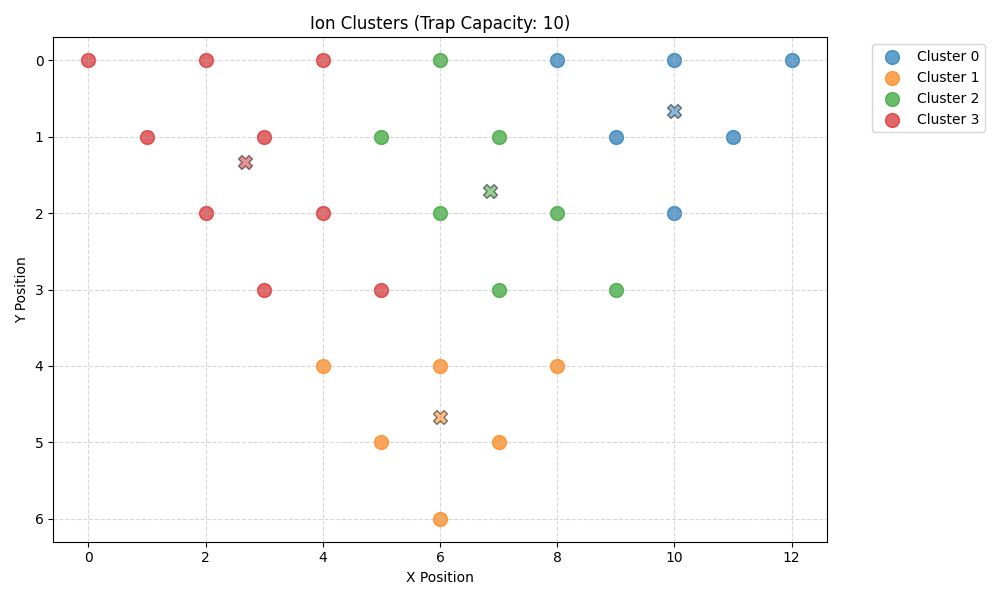
\includegraphics[width=\textwidth]{assets/clusters/tri_knn_clusters_tc=10_d=5.png}
     \caption{$k$-nearest-neighbour clustering, $k=3$}
     \label{fig:plot3}
\end{figure}

\begin{figure}[H]
    \centering
     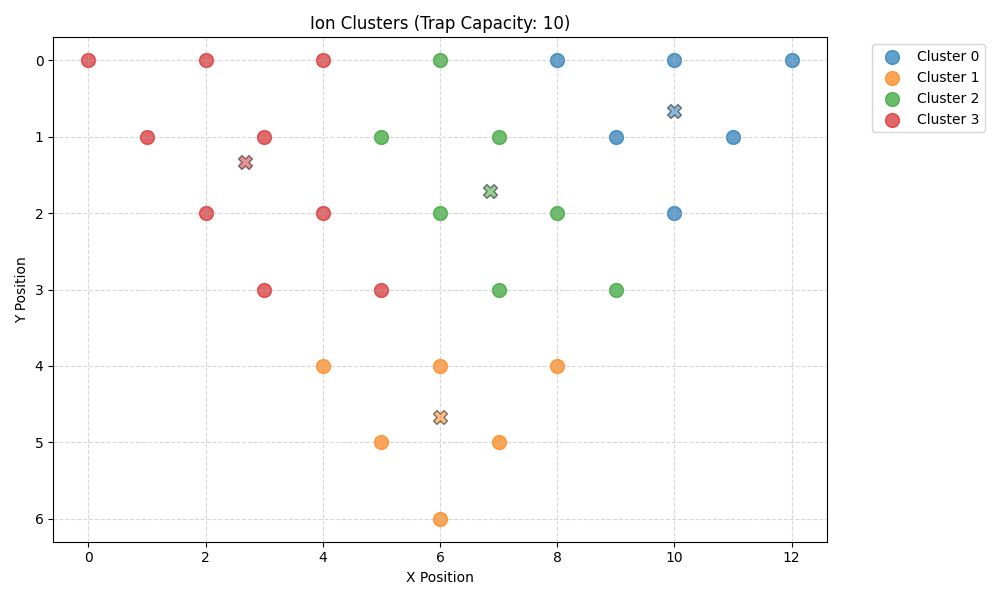
\includegraphics[width=\textwidth]{assets/clusters/tri_unbounded_nn_clusters_tc=10_d=5.png}
     \caption{Unbounded nearest-neighbour clustering}
     \label{fig:plot4}
\end{figure}

An interesting artifact of the framework clustering in Fig. \ref{fig:framework10} is observed in cluster 2, composed of three ions in the top left corner alongside a separated, singular ion towards the top middle. In comparison, the triangular clustering mechanisms preserve and form tighter clusters for the same top left corner. 

From these results, the bounded nearest-neighbour clustering demonstrates the tendency to form a larger number of clusters relative to other methods due to its tighter constraint on the search space in the merging stage. A potential experiment for later stages could be the effect of increasing the boundary threshold value on compilation metrics such as logical error rate and syndromic extraction time.

\section{Framework Changes}

In order to provide the functionality for compiling color codes, the entire pipeline required additional features and restructuring.

Changes were made to the pipeline incrementally as the project progressed through the stages.


\begin{itemize}
    \item Adapting simulator QCCD.circuit class to enable generation of available color code classes 
    \item Adapting simulator to differentiate between code types, utilising chromobius when a color code was used
    \item Adding methods that enabled processing of color code circuits, including setting up the required hardware from input hardware parameters.
    \item Providing flexibility in pipeline to choose the mapping methodology, used to compare effect of mapping strategies in the eval section 
    \item Test suite for integration and functional testing of color code generation and mapping strategies 
    
\end{itemize}
\section{Extension: The (4.8.8) Color Code}

Alongside the (6.6.6) color code, a stretch goal included the implementation of an alternative color code tessellation to provide a richer source of testing material to further validate the compiler and mapping methodologies. 

The primary challenge in implementing this color code was its complex geometry, greatly diverging from the uniformly tiled hexagons of the (6.6.6) color code. In addition to the difficulty of generating a single tiling, it was also necessary for the tiling mechanism to generalise to all possible input distances.
The (4.8.8) tile generation procedure was developed over several days of trial and error, by identifying underlying structural patterns, then identifying the base qubits and their respective face shapes to construct the topology relative to the base.  

\begin{figure}[htbp]
    \centering
    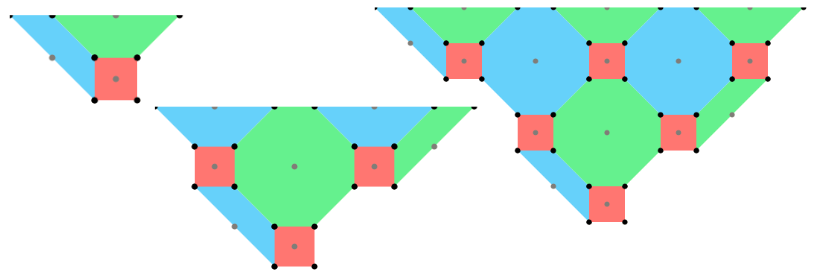
\includegraphics[width=0.75\linewidth]{assets/488colorcodes.png}
    \caption{Generated topology of the (4.8.8) color code}
    \label{fig:488colorcodes}
\end{figure}

The second challenge lay in the generation of the quantum circuit, where the syndrome extraction required finer detail, due to differing weight stabilizers that occurred in the code. 


\newpage
\section{Extension: Research Based Experiments}

On completion of the compilation pipeline for the color code, the framework is now able to process and evaluate the suitability of the code on various architectural QCCD designs. Naturally, this opens up the project towards researching some key questions.

\begin{itemize}
    \item \textit{What are the effects and suitability of different QCCD hardware topologies on color codes?}
    \item \textit{How does the choice of trap capacity influence logical error rates?} 
    \item \textit{What parameters or properties are the compilation time bottlenecks for color codes?}
    \item \textit{What specific architectural parameters provide the most promising path towards FTQC with color codes?}
\end{itemize}

For this section, the majority of the work was done in \mintinline{python}{JupyterNotebook}, using its interactive features to vary parameters by hand and run compilation experiments, alongside the generation of plots.




